\begin{figure}[htb]
    \centering
    % First TikZ picture
    \begin{tikzpicture}
        \begin{axis}[
            xlabel={$t / \mathrm{ms}$},
            ylabel={$i' / i'^* / \mathrm{A}$},
            axis lines=left,
            ymin=0, ymax=30,
            xmin=0, xmax=10,
            xtick={0,1,2,3,4,5,6,7,8,9,10},
            ytick={0,5,10,15,20,25,30},
            thick,
            smooth,
            no markers,
            height=7cm,
            width=0.99\textwidth,
            grid
            ]
            
            \addplot[signalblue, domain=0:10, samples=200] {24.5 * (1 - ((x-5)/5)^2)};
            
            \draw[thick, blue]
         %   (0,0) -- (0.48,2.35)
           % -- (0.5, 0.95) -- (0.935, 7.27)
           % -- (1.008, 2.5)
           -- (1.25,8.6) -- (1.388,12.2)-- (1.520,5.5) 
            -- (1.852,16.4)-- (2.044,8.3)
            -- (2.35,19.9) -- (2.58,11.3) 
            -- (2.82,22.7) -- (3.1,14.5) 
            -- (3.3,24.9) -- (3.6,17.2)
            -- (3.8,26.3) -- (4.1,19.5)  
            -- (4.2,27.2) -- (4.6,21) 
            -- (4.7,27.8) -- (5.15,21.8) 
            -- (5.2,27.9) -- (5.6,21.5) 
            -- (5.7,27.5) --(6.1,20.5) 
            -- (6.2,26.9) -- (6.6,18.7)
            -- (6.8,25.8) -- (7.1,16.3) 
            -- (7.3,24.2) -- (7.62,13.5)
            -- (7.84,21.9) -- (8.156,10.5) 
            -- (8.462,19)-- (8.68,7.5) 
            -- (8.942,15.1) -- (9.084,4.2) 
            -- (9.319,10.2) -- (9.58,1.8)  
            --  (9.9,4.2) -- (10,0);
            \end{axis}
    \end{tikzpicture}

    
    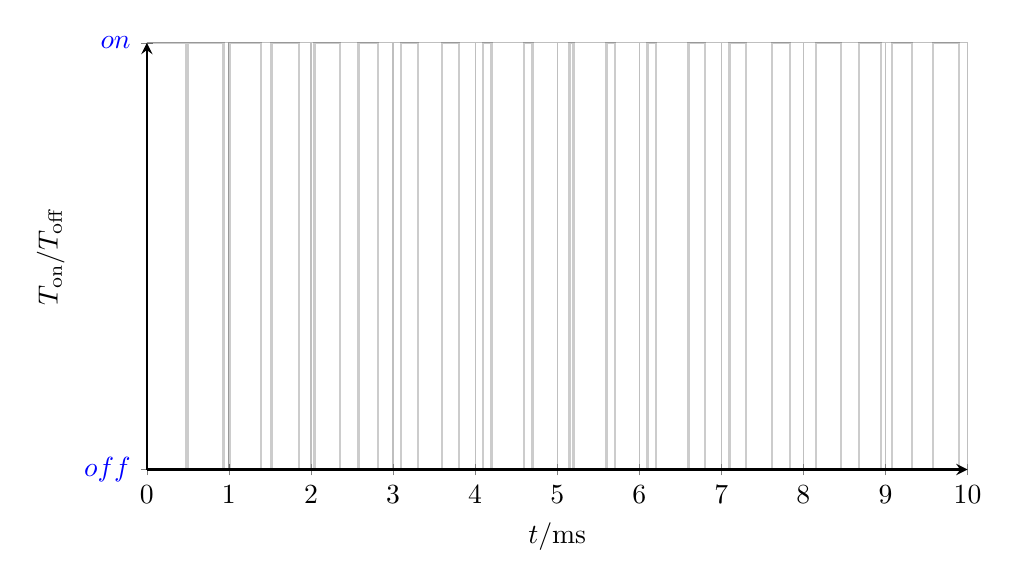
\begin{tikzpicture}
        \begin{axis}[
           % \hspace{1cm} % Grafiken um 2 cm nach rechts verschieben
            xlabel={$t / \mathrm{ms}$},
            ylabel={$T_\mathrm{on}/T_\mathrm{off}$},
            axis lines=left,
            ymin=0, ymax=1,
            xmin=0, xmax=10,
            xtick={0,1,2,3,4,5,6,7,8,9,10},
            ytick={0,1},
            yticklabels={{\color{blue}$off$},{\color{blue}$on$}},
            thick,
            smooth,
            height=7cm,
            width=0.99\textwidth,
            grid
            ]
    
            
            \draw[opacity=0.2] 
                (axis cs:0, 1) -- (axis cs:0.48, 1) -- (axis cs:0.48, 0) -- (axis cs:0, 0) -- cycle;
            
            \draw[opacity=0.2] 
                (axis cs:0.5, 1) -- (axis cs:0.935, 1) -- (axis cs:0.935, 0) -- (axis cs:0.5, 0) -- cycle;
    
            
            \draw[opacity=0.2] 
                (axis cs:1.008, 1) -- (axis cs:1.388, 1) -- (axis cs:1.388, 0) -- (axis cs:1.008, 0) -- cycle;
    
            
            \draw[opacity=0.2] 
                (axis cs:1.52, 1) -- (axis cs:1.852, 1) -- (axis cs:1.852, 0) -- (axis cs:1.52, 0) -- cycle;

            \draw[opacity=0.2] 
                (axis cs:2.044, 1) -- (axis cs:2.35, 1) -- (axis cs:2.35, 0) -- (axis cs:2.044, 0) -- cycle;

            \draw[opacity=0.2] 
                (axis cs:2.58, 1) -- (axis cs:2.82, 1) -- (axis cs:2.82, 0) -- (axis cs:2.58, 0) -- cycle;

            \draw[opacity=0.2] 
                (axis cs:3.1, 1) -- (axis cs:3.3, 1) -- (axis cs:3.3, 0) -- (axis cs:3.1, 0) -- cycle;

            \draw[opacity=0.2] 
                (axis cs:3.6, 1) -- (axis cs:3.8, 1) -- (axis cs:3.8, 0) -- (axis cs:3.6, 0) -- cycle;    

            \draw[opacity=0.2] 
                (axis cs:4.1, 1) -- (axis cs:4.2, 1) -- (axis cs:4.2, 0) -- (axis cs:4.1, 0) -- cycle;   

            \draw[opacity=0.2] 
                (axis cs:4.6, 1) -- (axis cs:4.7, 1) -- (axis cs:4.7, 0) -- (axis cs:4.6, 0) -- cycle; 

            \draw[opacity=0.2] 
                (axis cs:5.15, 1) -- (axis cs:5.2, 1) -- (axis cs:5.2, 0) -- (axis cs:5.15, 0) -- cycle;
                
            \draw[opacity=0.2] 
                (axis cs:5.6, 1) -- (axis cs:5.7, 1) -- (axis cs:5.7, 0) -- (axis cs:5.6, 0) -- cycle;

            \draw[opacity=0.2] 
                (axis cs:6.1, 1) -- (axis cs:6.2, 1) -- (axis cs:6.2, 0) -- (axis cs:6.1, 0) -- cycle;

            \draw[opacity=0.2] 
                (axis cs:6.6, 1) -- (axis cs:6.8, 1) -- (axis cs:6.8, 0) -- (axis cs:6.6, 0) -- cycle;
                
            \draw[opacity=0.2] 
                (axis cs:7.1, 1) -- (axis cs:7.3, 1) -- (axis cs:7.3, 0) -- (axis cs:7.1, 0) -- cycle;

            \draw[opacity=0.2] 
                (axis cs:7.62, 1) -- (axis cs:7.84, 1) -- (axis cs:7.84, 0) -- (axis cs:7.62, 0) -- cycle;

            \draw[opacity=0.2] 
                (axis cs:8.156, 1) -- (axis cs:8.462, 1) -- (axis cs:8.462, 0) -- (axis cs:8.156, 0) -- cycle;

            \draw[opacity=0.2] 
                (axis cs:8.68, 1) -- (axis cs:8.942, 1) -- (axis cs:8.942, 0) -- (axis cs:8.68, 0) -- cycle;

            \draw[opacity=0.2] 
                (axis cs:9.084, 1) -- (axis cs:9.319, 1) -- (axis cs:9.319, 0) -- (axis cs:9.084, 0) -- cycle;

            \draw[opacity=0.2] 
                (axis cs:9.58, 1) -- (axis cs:9.9, 1) -- (axis cs:9.9, 0) -- (axis cs:9.58, 0) -- cycle;

            
    
        \end{axis}
    \end{tikzpicture}
    

    \caption{Current i' and control signal for power transistor T.}
    \label{fig:Current i' control signal ex05}
\end{figure}
